\section{Results}
\label{S:w5}
 For data preparation and feature extraction, R programming language is used. All the classification algorithms, including pseudo-labelling and ResNet MLP were coded in Python programming language, using Keras library \cite{chollet2015keras} and its implementation of TensorFlow with GPU support \cite{tensorflow2015-whitepaper}. After preparing the data for the analysis, network configuration is optimized based on ResNet34, which is one of the most commonly used architectures, initially introduced in~\cite{he2016deep}. In this step, whether to add batch normalization and dropout layers, and number of nodes (neurons) in each hidden layer is determined, and the best configurations are selected for the next stage. The best configurations selected in the previous step will then be implemented in different architectures, with different sample rates of pseudo-label algorithm to find the final model. 
 \subsection{Tuning ResNet Configuration}
 The ResNet core of the model can be configured in various ways. Going through all the possible conditions would require a timely and computationally expensive search. In this section, we try to cover a range of possible configurations based on dropout layers, batch normalization layers, and number of nodes (neurons) in hidden layers:
 \begin{itemize}
     \item \emph{Batch Normalization:} By performing normalization for each training mini-batch, batch normalization makes normalization a part of the model architecture. It also can be used as a regularizer to replace dropout in some cases \cite{ioffe2015batch}. 
     \item \emph{Dropout:} Aiming at reducing overfitting in the models, dropout's key idea is to randomly drop units and their connections from the neural network during training \cite{srivastava2014dropout}. 
     \item \emph{Number of Neurons (nodes):} Efficient number of nodes in each hidden layer should be carefully investigated, as low number of nodes can cause underfitting, and using too many nodes may result in overfitting. For the ease of calibration and to limit the number of possible architecture, we assume that all hidden layers are similar and have an equal number of nodes.
 \end{itemize}
As presented in \cref{tab:total}, 16 configurations can be generated based on the possible combinations of the three items. Each configuration is named using a letter \textit{a, b, c, d} representing number of nodes in hidden layers, and a regularization ID, all provided in parentheses in front of the items. For instance, Config-a10 refers to a configuration having 5 nodes in each hidden layer (a), with regularization ID \textit{10}, meaning that batch normalization is conducted before all layers (1) and no dropout layer is used (0).  All the configurations are implemented and tested in a supervised manner on ResNet34, which appears to be a good starting architecture, as it offers good performance in spite of less time complexity and model size comparing to other architectures in the original paper~\cite{he2016deep}. Performance of these configurations is compared after 500 number of epochs, with 20\%  of the data used as the validation set. For time-saving purposes, the accuracy of the models in this stage is not estimated using 10-fold cross validation. Batch size for all the tests is set equal to 32, and considering its successful performances in deep learning literature~\cite{kingma2014adam}, Adam method is used as the optimizer. Finally, best model will be selected for the next step, which will be the implementation of the core in a semi-supervised manner in different architectures.

Accuracy of ResNet34 on training set and validation set for all configurations, along with their respective run time and gap percentage between training and validation accuracy are provided in \cref{tab:acc}. \cref{fig:acc} presents a comparative bar plots of the configurations. As shown in \cref{fig:acc}a and \cref{fig:acc}b, all configurations having 20 nodes in their hidden layers, are performing worse on training and validation sets, than their counterpart configurations with 15 nodes in hidden layers. Thus, more nodes are not added to hidden layers. According to the results, top configurations based on accuracy of training and validation sets are: \textbf{c00}, \textbf{d00}, and \textbf{b00}. In all these three configurations, batch normalization and dropout layers are removed. The effect of removing regularization layers is clearly observable in gap \% of training and validation accuracy: despite high accuracy in training and validation sets, the gap between these two accuracies in three configurations are relatively high. The main purpose of batch normalization and dropout layer is to prevent overfitting over the training set. High accuracy on training data (over 95\% in three cases) and relatively large gap between training and validation accuracy is a sign of overfitting in these configurations. Configurations with regularization ID \textit{01}, in which dropout is used for regularization, have a maximum accuracy of 65\% on both training and validation sets. Considering high gap between validation and training accuracy, overfitting occurred in these configurations.  Adding batch normalization layers in configurations with regularization ID \textit{11}, helped to reduce overfitting slightly. However, the accuracies remained low.

\begin{table*}[t]
    \caption{Different ResNet34 Configurations}
    \centering
    \scalebox{0.7}{
    \small\addtolength{\tabcolsep}{-4pt}
    \begin{tabular}{|l|l|l|l|l|l|l|l|l|l|l|l|l|l|l|l|l|}
    \hline
       \textbf{Configuration}  & \textbf{a00} & \textbf{a01} & \textbf{a10} & \textbf{a11} & \textbf{b00} & \textbf{b01} & \textbf{b10} & \textbf{b11} & \textbf{c00} & \textbf{c01} & \textbf{c10} & \textbf{c11} &\textbf{d00}&\textbf{d01}&\textbf{d10}&\textbf{d11}  \\
       \hline\hline
    
         \textbf{Training accuracy (\%)}&85.7 &54.2 & 60.3  &54.7& 95.6 &60.7 &72.9& 55.7&96.6 &63.7 &81.1& 56.7& 96.9&65.1&79.3&  58.6 \\
    
         \textbf{Validation accuracy (\%)}&76.5 &51.2 & 52.9 & 51.2 & 80.6 &53.6&68.5 & 50.6&84.7 &52.9& 79.4& 51.2& 82.9&52.9&75.9& 51.2\\
        \textbf{\% of difference}& 11&6  & 12 &6 &16 &12 &6&9&12 &17 &2 &10  &14&19&4&13\\
         
    \hline
        \textbf{Run Time (s)}&698&889&1195&1895 & 783&820&985&2107 &703&875&1249&1752 & 662&915&1186&1999\\
        \hline
    
    \end{tabular}}

    \label{tab:acc}
\end{table*}
On the other hand, configurations with regularization ID \emph{10}, appear to have satisfying performance on both aspects: least gap between training and validation accuracy, and acceptable prediction accuracy on training and validation data.  Batch normalization in these configurations makes the networks not requiring dropout for regularization~\cite{ioffe2015batch}.

\begin{figure*}
    \centering
    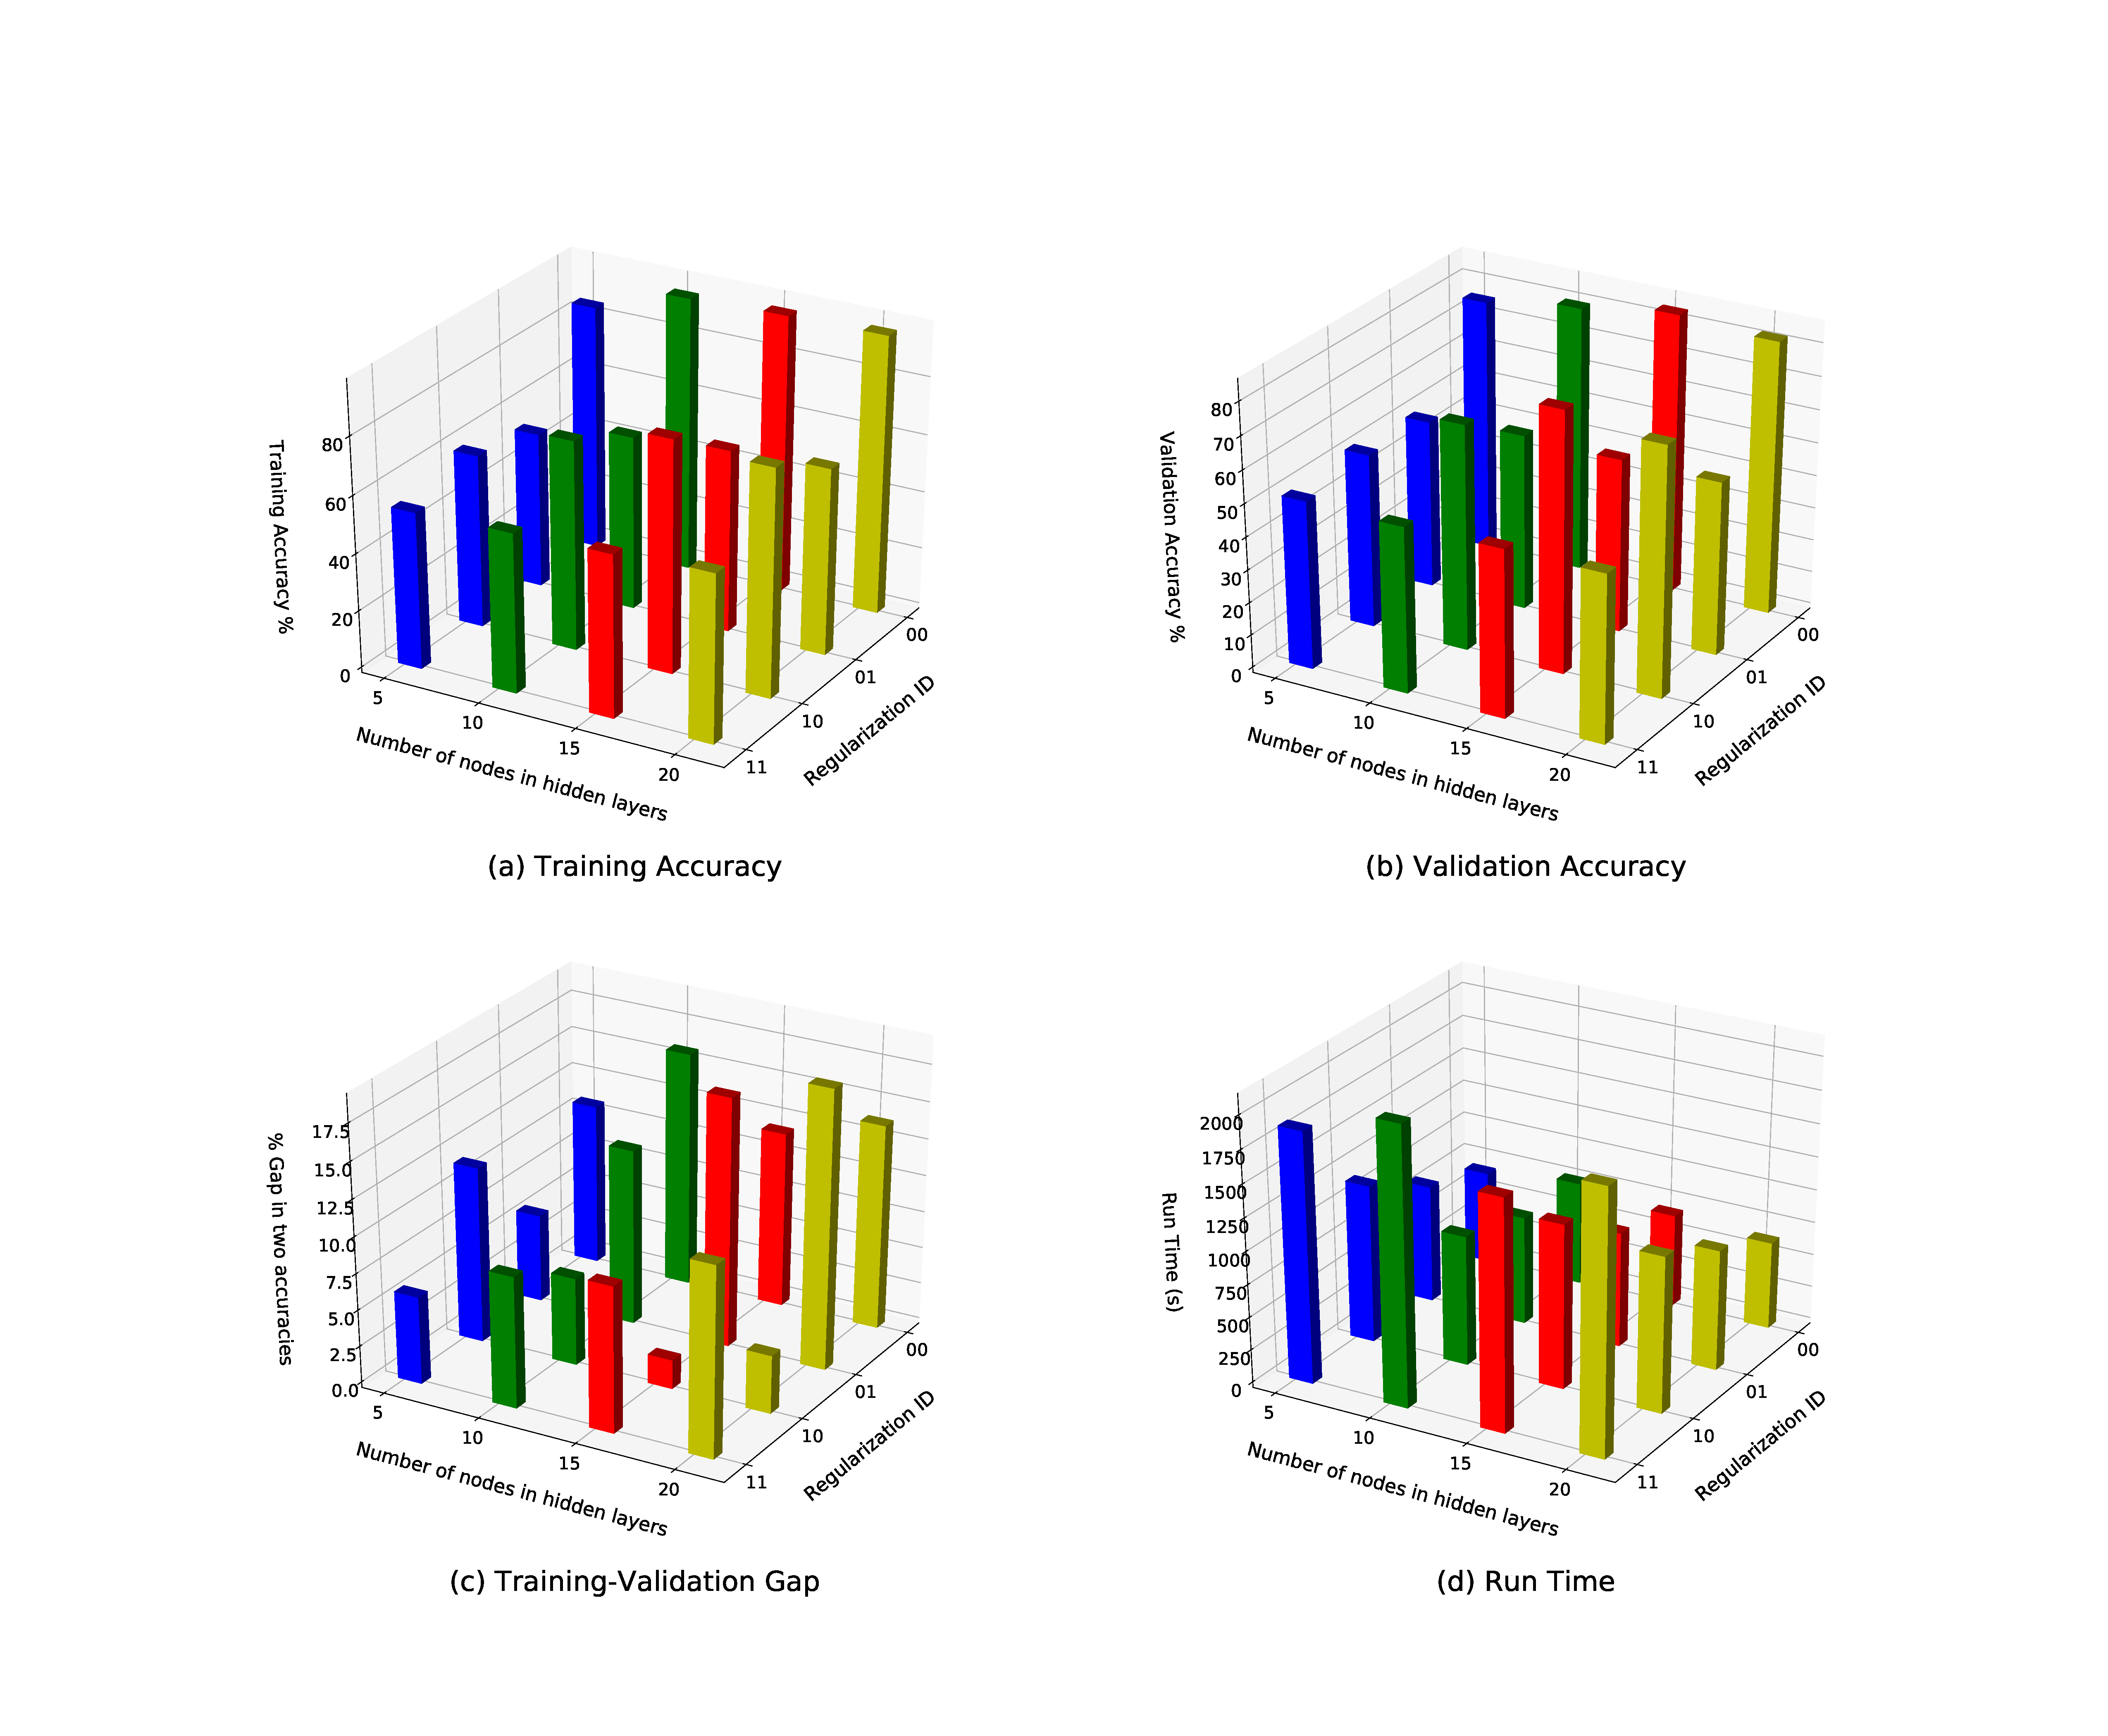
\includegraphics[scale=0.15]{chapter_2/figures/conf.pdf}
    \caption{Comparing different ResNet34 Configurations }
    \label{fig:acc}
\end{figure*}
Considering various aspects described above, \emph{c10} configuration is selected as the candidate in this step to be fed into our pseudo-label algorithm in the next stage.
To further investigate configurations, training run times are compared. As it is expected, adding dropout and batch normalization layers significantly increases the time it takes to run the code. However, for \emph{c10}, which is the configuration selected, it takes an affordable time of 1249 seconds to be trained by 500 epochs, on a 1.6GHz dual-core Intel Core i5 processor. \cref{fig:epoch} shows the trend of accuracy in training and validation set over 500 number of epochs for \emph{c10}.
\begin{figure}[t]
    \centering
    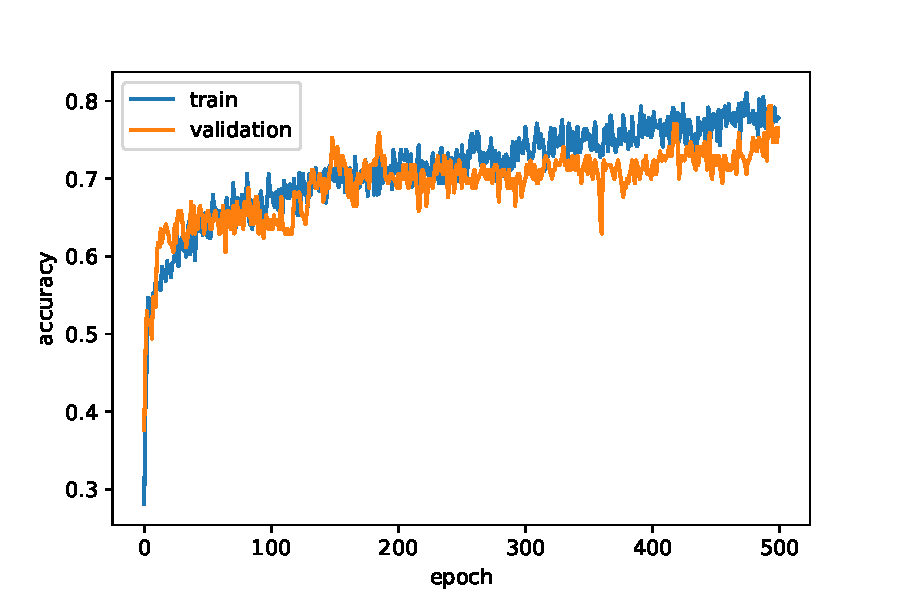
\includegraphics[scale=0.55]{chapter_2/figures/c10.pdf}
    \caption{Training and validation performance of c10}
    \label{fig:epoch}
\end{figure}
\begin{center}
\begin{table*}[ht]
\caption{Parameters of core ResNet architecture, values in () are for naming purposes}
\scalebox{0.85}{
\setlength\extrarowheight{2pt}
\centering
\begin{tabular}{|l|*{32}{p{\Wlena}|}}
\hline
\textbf{Configuration Item}           & \multicolumn{32}{c|}{\textbf{Explored Values}}\\
\hline\hline
Number of nodes in hidden layers & \Wmcii{5 (a)} & \Wmcii{10 (b)} & \Wmcii{15 (c)} & \Wmcii{20 (d)}  \\  
\hline
Batch Normalization & \Wmciii{No (0)} & \Wmciii{Yes (1)}  \\
\hline
Dropout Layer & \Wmciii{No (0)} & \Wmciii{Yes (1)}  \\
\hline
\end{tabular}}
\label{tab:total}
\end{table*}
\end{center}
 \subsection{Model Sensitivity Analysis}
 In the second stage for model calibration, configuration found in the previous section is fixed to find the best model architecture. In each architecture, number of layers within a building block is set to be equal to either 2 or 3 similar to~\cite{he2016deep}. In addition, different number of building blocks within the ResNet MLP architecture are tested. Architectures are developed mainly based on their presence in~\cite{he2016deep}: For two-layer building block architectures, ResNet18 and ResNet34 and for three-layer building block architectures, ResNet50, ResNet101, and ResNet152 are tested. In addition, to explore other architectures, ResNet10 for two-layer building block networks, and ResNet74 and ResNet122 for three-layer building block networks are developed. The number in the model names represents the number of layer in that model. For instance, ResNet101 consists of 33 building blocks, each having three layers, plus an input and an output layer. On the pseudo-label part of the model, 6 sample rates are tested for each architecture: 0, 0.2, 0.4, 0.6, 0.8 and 1. Having a sample rate of 0 means that unlabelled data are not fed into the model, and pseudo-labelling part is ignored. By using a 0 sample rate, we will be able to better compare the performance of the classifier in a supervised and semi-supervised manner. On the other side, a sample rate of 1 means inserting all unlabelled data into the algorithm and pseudo-labelling them at once.  Model evaluation in this step is conducted using 10-fold cross-validation: dataset is randomly divided into 10 groups or folds. The first fold will be used as validation set, and the other 9 folds will be used to train the classifier. This procedure is repeated 10 times, having a different fold as validation set each time. Different model architectures are tested to find the optimal model with the best performance in 10-fold cross-validation. The best model, based on the total accuracy will then be selected and applied on a test set consisting of separated labelled data not used in the training procedure.   The number of epochs in training the model was set to be 1000 for all architectures. All the models are trained on a Core i7 4GHz CPU and a 16.0 GB memory.  
 
 Compared to plain non-residual architectures, all ResNet-based architectures showed significantly better performances than plain 34-layer MLP. A low accuracy of 56\% is achieved by using a deep non-residual network with 34 layers, which shows the power of adding identity shortcut connections to the network. \cref{fig:results2} depicts the accuracy of different architectures for models with a two-layer building block and three-layer blocks are compared.  As it can be inferred from the figures, performance of ResNet MLP architectures in a supervised manner, i.e. a sample rate of 0\%, appears not to be improving while increasing the number of hidden layers. ResNet18 for instance performs better than its deeper counterpart, ResNet32, for 2-layer building block models. Similarly, ResNet74 performs better than ResNet101 and ResNet122. However, adding the pseudo-label algorithm with a sample rate of 20\% results in a better performance of deeper networks. Specifically, for networks with more building blocks, improvement in performance using pseudo-labels appears to be more significant. For ResNet122 for instance, the accuracy increases by around 5\% with 20\% sample rate of pseudo-labels, whereas for ResNet10, the increase is less than 1\%, and for ResNet18, semi-supervised learning does not help to improve the performance. It can be concluded that having more building blocks, in general, tends to cause more overfitting, which is addressed by adding pseudo-labelled data to the model. 
 
 For sample rates greater than 20\%, the fluctuations in the accuracy increases and does not follow a predictable trend. Thus, sample rate of 20\% is selected as the optimum number for pseudo-labelling. On the other side, performance of the model in the deepest architecture, ResNet152 starts decreasing compared to ResNet122, which made us stop adding more hidden layers to the architecture. In conclusion, ResNet122 with a sample rate of 20\% is selected as the best model for classifying mode of transport using collected Wi-Fi data. Regarding the training time of the selected framework, a 10-fold cross-validation on the model takes around 4 hours to run, meaning an estimated average of 24 minutes per classifier.
\begin{figure}[!ht]
  \centering
  \begin{tabular}{@{}c@{}}
    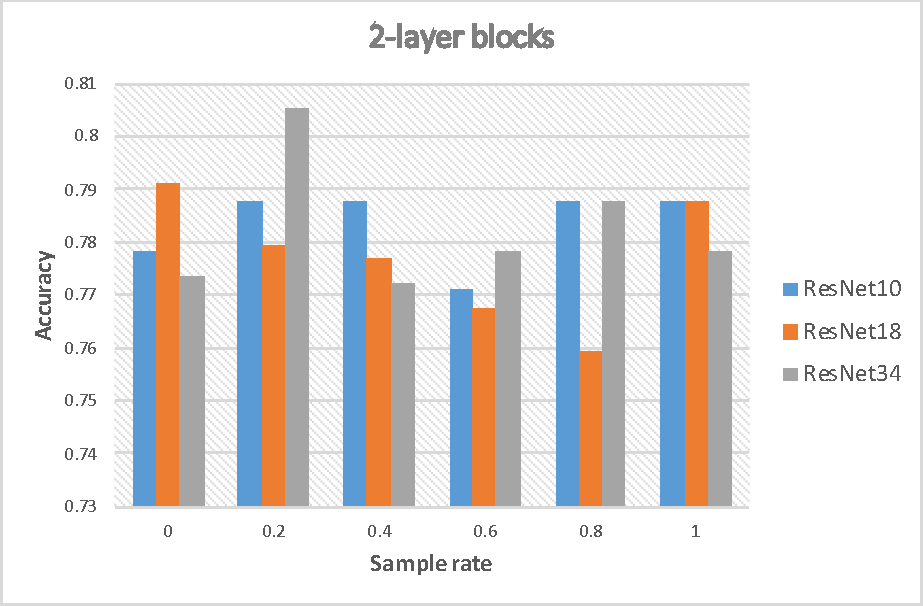
\includegraphics[width=0.8\linewidth]{chapter_2/figures/2layer.pdf} \\[\abovecaptionskip]
    \small (a) 2-layer building blocks
  \end{tabular}

  \vspace{\floatsep}

  \begin{tabular}{@{}c@{}}
    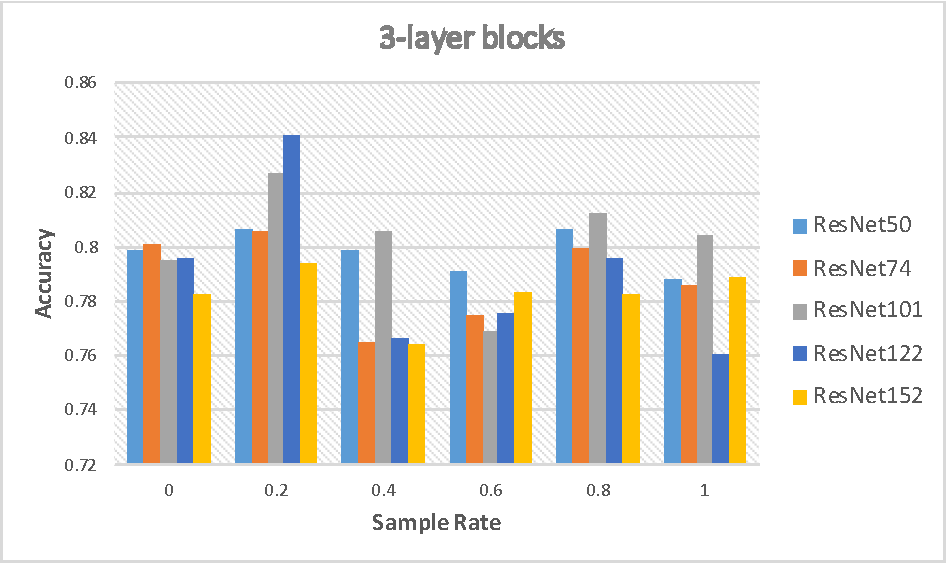
\includegraphics[width=0.8\linewidth]{chapter_2/figures/3layer.pdf} \\[\abovecaptionskip]
    \small (b) 3-layer building blocks
  \end{tabular}

  \caption{Model sensitivity analysis for number of building blocks and sampling rate}\label{fig:results2}
\end{figure}

 
\subsection{Final Model Accuracy Analysis}
The highest accuracy of the model, as it is depicted in \cref{fig:results2} is achieved in ResNet122 with a sample rate of 20\%. With an 84.1\% accuracy in 10-fold cross-validation, the model outperforms all the other architectures, supervised and semi-supervised, residual and non-residual. In \cref{tab:ConMat}, confusion matrix of this architecture is depicted based on a test set. Recall and precision of each mode of transport in confusion matrix are estimated based on a 20\% sample of labelled data, which was not used in the training procedure. Test set includes 170 rows of labelled data, including 43 walking, 41 biking and 86 driving trips. As provided in the table, the model successfully predicts all three modes of transportation with an precision of over 80\%. Among modes, driving has the most accurate recall and precision, despite the fact that both data collection experiments are conducted in congested urban areas, where the speed of vehicles are not significantly higher than bikes and pedestrians. Unlike commonly used mode classification methods which rely merely on features such as speed to distinguish trips, our model has benefited from higher level features with the help of very deep residual networks.

The lowest precision in the confusion matrix belongs to bikes. Biking and driving modes share many similar features, particularly in congested urban areas with signalized intersections. Thus, relatively low precision of biking can be explained. As it can be seen in \cref{tab:ConMat}, 8 driving trips that are incorrectly predicted as biking, play the main role in low accuracy of biking. These 8 trips consist less than 10\% of the driving trips. 
\begin{table}[!ht]
\centering
\caption{Confusion Matrix of ResNet122 with 20\% sample rate} 
\small
\begin{tikzpicture}[
box/.style={draw,rectangle,minimum size=1.1cm,text width=1.1cm,align=center}]
\matrix (conmat) [row sep=.1cm,column sep=.1cm] {
\node (1) [box,
    label=left:\textbf{Walking},
    label=above:\textbf{Walking},
    ] {35};
&
\node (2) [box,
    label=above:\textbf{Biking},
    ] {3};
&
\node (3) [box,
    label=above:\textbf{Driving},
    ] {5};
&
\node(4) [label=above:\textbf{Total}]{43};
&
\node(5) [label=above:\textbf{Recall\%}]{81.4};
\\
\node (6) [box,
    label=left:\textbf{Biking},
    ] {2};
&
\node (7) [box,
    ] {33};
&
\node (8) [box,
    ] {6};
    &
\node(9) {41};
 &
\node(10) {80.5};
\\
\node (11) [box,
    label=left:\textbf{Driving},
    ] {5};
&
\node (12) [box,
    ] {8};
&
\node () [box,
    ] {73};
&
\node(14) {86};
 &
\node(15) {84.9};
\\
\node (16) [
    label=left:\textbf{Total},
    ] {42};
&
\node (17) {44};
&
\node (18)  {84};
&
\node (9)  {170};
\\
\node (10) [
    label=left:\textbf{Precision},
    ] {83.3};
&
\node (8) {75.0};
&
\node (9)  {86.9};
\\
};
\node [rotate=90,left=.1cm of conmat,anchor=center,text width=1.5cm,align=center] {\textbf{Actual}};
\node [above=.1cm of conmat,align=center,anchor=center] {\textbf{Prediction}};
\end{tikzpicture}
\label{tab:ConMat}
\end{table}
Due to a higher volume of vehicles in the area, our dataset consist of approximately 50\% driving trips. The higher number of driving trips in the data can result in the model to develop a tendency to be fitted better for this mode. This tendency led our framework to predict 5 walking trips (11\% of all walking trips) as driving. For a similar reason, 6 bike trips (14.6\% of all bike trips) are incorrectly predicted as driving. Despite all the above-mentioned inaccuracies, the model has been capable of predicting the correct mode of transportation with a satisfying accuracy of 84.1\% for all the trips based on 10-fold cross-validation results, and 82.9\% on the test set. Another measure of test accuracy, F-score, which is defined as the harmonic average of precision and recall, were calculated to be 0.82, 0.78 and 0.86 for walk, bile and driving mode respectively. The average F-score of the modes appears to be 0.82.